\let\negmedspace\undefined
\let\negthickspace\undefined
\documentclass[journal]{IEEEtran}
\usepackage[a4paper, margin=10mm, onecolumn]{geometry}
\usepackage{lmodern} % Ensure lmodern is loaded for pdflatex
\usepackage{tfrupee} % Include tfrupee package

\setlength{\headheight}{1cm} % Set the height of the header box
\setlength{\headsep}{0mm}  % Set the distance between the header box and the top of the text

\usepackage{gvv-book}
\usepackage{gvv}
\usepackage{cite}
\usepackage{amsmath,amssymb,amsfonts,amsthm}
\usepackage{algorithmic}
\usepackage{graphicx}
\usepackage{float}
\usepackage{textcomp}
\usepackage{xcolor}
\usepackage{txfonts}
\usepackage{listings}
\usepackage{enumitem}
\usepackage{mathtools}
\usepackage{gensymb}
\usepackage{comment}
\usepackage[breaklinks=true]{hyperref}
\usepackage{tkz-euclide} 
\usepackage{listings}
% \usepackage{gvv}                                        
\def\inputGnumericTable{}                                 
\usepackage[latin1]{inputenc}                                
\usepackage{color}                                            
\usepackage{array}                                            
\usepackage{longtable}                                       
\usepackage{calc}                                             
\usepackage{multirow}                                         
\usepackage{hhline}                                           
\usepackage{ifthen}                                           
\usepackage{lscape}
\usepackage{tikz}
\usetikzlibrary{patterns}

\begin{document}

\bibliographystyle{IEEEtran}
\vspace{3cm}

\title{2.9.15}
\author{EE25BTECH11064 - Yojit Manral}

\maketitle
% \maketitle
% \newpage
% \bigskip
{\let\newpage\relax\maketitle}
\renewcommand{\thefigure}{\theenumi}
\renewcommand{\thetable}{\theenumi}
\setlength{\intextsep}{10pt} % Space between text and float

\textbf{Question:}\\
If the points $\vec{A}\brak{2,0}$, $\vec{B}\brak{6,1}$, and $\vec{C}\brak{p,q}$ form a triangle of area 12 square units(positive only) and
\begin{align}
    2p + q = 10
\end{align}
then find the values of p and q.

\textbf{Solution:}\\
\begin{table}[h!]    
  \centering
  \begin{tabular}[12pt]{ |c| c|}
    \hline
    \textbf{Points} & \textbf{Name}\\ 
    \hline
	\myvec{7\\10} & Point $\Vec{A}$ \\
    \hline 
	\myvec{-2\\5} & Point $\Vec{B}$\\
    \hline
	\myvec{3\\4} & Point $\Vec{C}$\\
    \hline
\end{tabular}
  \caption{List of Points}
  \label{Table_1}
\end{table}\\

$\rightarrow$ The are of the given $\triangle$ABC can be given by
\begin{align}
    Area(\text{ABC}) &= \frac{1}{2} \left| \myvec{2 & 6 & p\\0& 1 & q\\1 & 1 & 1} \right| \\
    2 \times Area(\text{ABC}) &= 2 \times \left| \myvec{1 & q\\1 & 1} \right| - 6 \times \left| \myvec{0 & q\\1 & 1} \right| + p \times \left| \myvec{0 & 1\\1 & 1} \right| \\
    &= 2(1-q) - 6(0-q) + p(0-1) \\
    &= 2 + 4q - p \\
    Area(\text{ABC}) &= 12 \\
    \left| 4q -p + 2 \right| &= 24 \\
    4q - p &= \pm 24 - 2
\end{align}

$\rightarrow$ From (1) and (8), we get

\begin{align}
    \myvec{2 & 1\\-1 & 4} \myvec{p\\q} &= \myvec{10\\\pm 24 - 2} \\
    \myvec{p\\q} &= \myvec{2 & 1\\-1 & 4}^{-1} \myvec{10\\ \pm 24 - 2} \\
    &= \frac{1}{9} \myvec{4 & -1\\1 & 2} \myvec{10\\ \pm 24 - 2} \\
    \myvec{p\\q} = \myvec{2\\6} &\text{ or } \myvec{p\\q} = \myvec{22/3\\ -14/3}
\end{align}

\begin{figure}[h!]
   \centering
   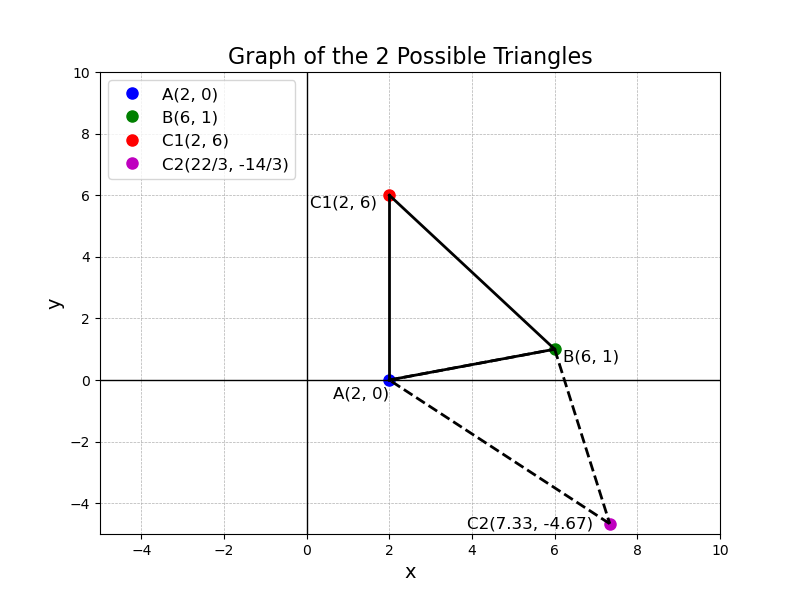
\includegraphics[width=\linewidth]{figs/01.png}
   \caption{Plot of points and triangles}
   \label{Plot_1}
\end{figure}
\end{document}
